\documentclass[a4paper,12pt,pre,superscriptaddress]{revtex4}
\usepackage{latexsym} 
%\usepackage{helvet}
%\usepackage{times}
%\usepackage[applemac]{inputenc}
\usepackage{amsmath} 
\usepackage{setspace}
\usepackage{color}
\usepackage{hyperref}
\usepackage{fancyhdr}
\usepackage{graphicx}
\usepackage{wrapfig}
%%%\usepackage{ulem} % to get the \sout command for editing

\newcommand{\rev}[1]{\textcolor{red}{#1}}

\usepackage[margin=2cm]{geometry}

%\bibliographystyle{authordate1}


\begin{document} 

\title{Combined collapse by bridging and self-adhesion in a
  prototypical polymer model inspired by the bacterial nucleoid.}
%%% maybe not a good idea to mention nucleoid in title ??

\author{Vittore~F. Scolari}
%%
\affiliation{Sorbonne Universit\'es, UPMC Univ Paris 06, UMR 7238,
  Computational and Quantitative Biology, 15 rue de l'\'{E}cole de
  M\'{e}decine Paris, France}
%
\affiliation{CNRS, UMR 7238, Paris, France}
%%
% \author{Bruno Bassetti} 
% %
% \affiliation{Universit\`a degli Studi di
%   Milano, Dip.  Fisica, Via Celoria 16, 20133 Milano, Italy}
% \affiliation{I.N.F.N. Milano, Via Celoria 16, 20133 Milano, Italy}
% 
%
\author{Vincenzo~G. Benza}
%
\affiliation{Dipartimento di Fisica e Matematica, Universit\`a
  dell'Insubria, Como, Italy} 
%
\author{Marco Cosentino Lagomarsino}
%%
\affiliation{Sorbonne Universit\'es, UPMC Univ Paris 06, UMR 7238,
  Computational and Quantitative Biology, 15 rue de l'\'{E}cole de
  M\'{e}decine Paris, France}
%
\affiliation{CNRS, UMR 7238, Paris, France}

\begin{abstract}
  Recent results in \emph{E.~coli} indicate that the chromosome feels
  a self-attracting interaction of osmotic origin, and is condensed in
  compartments by bridging interactions.
%%
  Motivated by these findings, we define a generic framework combining
  the two ingredients (and ignoring others) to characterize their
  joint effects. Specifically, study a a simple polymer physics
  computational model with weak ubiquitous short-ranged self
  attraction and sparse stringer bridging interactions.  Combining
  theoretical arguments and simulations, we study the general
  phenomenology of polymer collapse induced by these dual
  contributions, in the case of regularly-spaced bridging.
%
  Our results characterize the competition between the classical
  collapse from uniform interactions and loop-mediated collapse from
  bridging in a combined phaase diagram.
%
  \textbf{ QUALCOSA DI PIU' SPECIFICO SU DIAGR DI FASE ?}
%
  Additionally, we show that bridging can induce stable
  compartmentalized domain. In these configurations, different
  ``cores'' of bridging proteins are kept separated by star-like
  polymer loops in an entropically favorable multi-domain
  configuration, with a mechanism that parallels micellar polysoaps.
%%
  Such compartmentalized domains are self-organized, and do not need
  any specific interactions driving their segregation.  Domains can be
  stable also in presence of uniform attraction, as long as the
  uniform collapse is above its theta point.
% %%%
\end{abstract}


\maketitle

\setstretch{1}


% possibily referee: Rosa, Marenduzzo, McLeish, Cook, Peter Olmsted,

\section{Introduction} 

%

It is now clear that bacterial chromosomes (which exist in the cell in
a mesoscopic dynamic complex composed of DNA, RNA and proteins called
``nucleoid'') are highly organized within cells. The conformational
properties of the folded genome are essential for the processes of
replication, transcription (and thus regulation of gene expression),
segregation~\cite{Benza2012,Dillon2010,Muskhelishvili2010}.


%%%% NAPS -> BRIDGING
Focusing on \emph{E.~coli}, the chromosome is a single circular
molecule of about $4.7$ million base pairs (Mbp) ($\approx1.5$
mm)~\cite{Trun1998,Stavans2006}. Nucleoid associated proteins, or
``NAPs'' (such as Dps and transcription factors Fis, H-NS, IHF, HU,
and condensin MukBEF), can modify the shape of the DNA both at local
and global levels~\cite{Dillon2010,LNW+06,Ohniwa2011}.
%
Of particular interest are bridging interactions~\cite{Wiggins2009}
(possible at least from Fis, H-NS, and MukBEF), which can in principle
induce looped domain formation, through mechanisms that are believed
to be important also for eukaryotes~\cite{Brackley2013,Barbieri2013b}.
For example, the NAP H-NS is explicitly reported to form a small set
of foci in the cell, bringing together distant binding
sites~\cite{Wang2011a}, 
%%% which are distributed non-uniformly along the
%%% genome~\cite{Scolari2011,Kahramanoglou2011}
and to reduce the size of purified
nucleoids~\cite{Thacker2013}.
%%
RNA polymerase, the DNA-binding enzyme responsible for gene
transcription, might also concentrate into transcription foci or
``factories,'' affecting the nucleoid structure by bringing together
distant loci~\cite{JC06,GHH+05}.


%%%% COMPACTION FROM OSMOTIC COLLAPSE
The \emph{E.~coli} nucleoid, with a linear size of $1.5$mm, occupies a
well-defined region of the cell, with a volume of 0.1-0.2
$\mu$m$^3$ (the bare DNA volume is about a factor 20-30
smaller)~\cite{Stavans2006}.  Strong nucleoid compaction into a
structure that does not fill the volume of the cell is experimentally
observed \emph{in vivo}~\cite{Zim06b-a,HadizadehYazdi2012}. %
The degree of compaction is modulated by the cell's growth conditions and
in response to specific external cues.  Rather than confinement from
the cell boundaries, the dominant force for this compaction is likely
to come from self-attraction due to molecular crowding and forces of
entropic origin effectively causing a short-ranged
self-attraction~\cite{Odi98,Vries2010}. This self-adherent polymer
organization is consistent with both \emph{in vivo}
observations~\cite{HadizadehYazdi2012,Fisher2013} and \emph{in vitro}
experiments~\cite{Pelletier2012} with purified nucleoids.
%
Note that compaction from bridging alone is not likely to be
responsible of this behavior, as cytoplasm-free nucleoids are larger
than cells~\cite{Pelletier2012,Wegner2012,Thacker2013}.
%
A sub-Rouse viscoelastic dynamics of individual loci, whose mean
apparent diffusion varies with chromosomal
coordinates~\cite{Javer2013,Weber2010} suggests that (i) a simple
polymer model is not likely to fully capture nucleoid organization
(ii) the organization and dynamics of inter-loci tethering might also
be complex.

%%% NOT EQUILIBRIUM GLOBULE
Importantly, the state of the nucleoid is far from being an amorphous
mass, randomly organized, such as e.g., one expects from a classical
equilibrium collapsed globule~\cite{Mirny2011}. On the contrary,
folded object with persistent mesosocopic features, including a linear
ordering of loci within the cell an overall coiled
shape~\cite{WLP+06,Wiggins2010,HadizadehYazdi2012,Fisher2013,Pelletier2012}.
%%%% MACRODOMAINS
In these respects, one important feature of the \emph{E.~coli}
chromosomes are so-called ``macrodomains''~\cite{VPR+04,MRB05,EB06}
often described as isolated compartments. Such domains are roughly
replichore-symmetric, i.e., mirror the order of replication of the
\emph{E.~coli} genome, from the replication origin locus, oriC, to the
terminus region, Ter). Evidence for such
compartmentalization~\cite{VPR+04} comes from the recombination
frequency between loci (which is proportional to the probability that
the two chromosomal segments come into contact within the cell),
showing a non uniform pattern.
%
Four macrodomains of a few hundred Kb in size have been identified,
which divide the chromosome into six contiguous
regions~\cite{Dame2011,Benza2012}.  Subsequent studies have confirmed
the presence of macrodomains using fluorescently labelled
loci~\cite{EMB08,EB06,LMB+05}. The Ter macrodomain appears to be
condensed by a single DNA-binding protein, MatP, which has a small set
of specific binding sites in the Ter region~\cite{Mercier2008}.
%%
%%% junier macrodomains drive segregation
A recent modeling work has implicated the differential condensation
levels by macrodomains, together with the targeting of the Ori and Ter
regions to specific subcellular positions, to the generation of the
chromosome segregation pattern observed \emph{in
  vivo}\cite{Junier2013}.

%%% SUPERCOILING -> BRANCHING  menzionato ma poi trascurato
Additionally, nucleoids are composed of topologically unlinked dynamic
domain structures, due to supercoiling (torsional constraints
generated by active processes and frozen by bridging) forming
plectonemes and toroids~\cite{Trun1998}, and stabilized by
nucleoid-associated proteins, auch as Fis and H-NS. This combination
of effects gives the chromosome a looped
shape~\cite{Postow2004,Skoko2006,Kavenoff1976}, where the loops form a
tree of plectonemes. Supercoiling and nucleoid organization affect
gene expression~\cite{Breier2004,Postow2004,Dillon2010}.
%%
The level of supercoiling is tightly regulated by the cell, and it can
be changed by the action of specific enzymes such as topoisomerases
and gyrases.


%%%% Hi-C studies [dove entra??]
Sequencing techniques (though relying on population averages) give
further insight into the folding of bacterial chromosomes.
High-throughput Chromosome Conformation Capture (3C) techniques have
been used to determine the global folding architecture of the
\emph{C.~crescentus} swarmer cell genome~\cite{Le2013,Umbarger2011},
which is easier to access experimentally than \emph{E.~coli}, due to
the well-characterized polar tethering of the chromosome and 
%
the more practicability of cell syncronization.
%
These data show a chromosomal fiber-like organization, linearly
ordered in a compressed ring-like fiber, and taking an eight shape
inside the cell.
%
Higher-resolution data~\cite{Le2013} also show spatial domains of
interacting, and exhibit a hierarchical nested organization over a
range of length scales ($\sim50-200$ Kb). These domains are stable
throughout the cell cycle and are reestablished concomitantly with DNA
replication.  Additionally, domain boundaries co-occur with
highly-expressed genes, and the domain organization is enabled by
transcription. Such domains are hypothesized to be composed of
transcription-induced supercoiled plectonemes arrayed into a ``bottle
brush'' fiber.
%%
Regarding \emph{E.~coli}, the current resolution appears too low
\cite{Cagliero2013} to draw any specific conclusions, but finer-scale
experiments are expected to appear soon.



%%%% Our Work 
While the bridging and loop-forming interactions are sometimes
incorporated in polymer models of the bacterial chromosome
\cite{Junier2013,Fritsche2012,Heermann2012}, they are 
%%
Here, we set out to investigate how the combination of bridging and
homogeneous collapse in a generic polymer physics (equilibrium)
framework, using computer simulations and with the help of theoretical
mean-field and scaling arguments.
%%
Rather than an explicit model for the chromosome, our intent is to
generically explores the consequences of these ingredients, in order
to help more realistic model development and to link the phenomenology
with the vast existing knowledge in polymer physics.
%%
In this spirit, we deliberately ignore the role of supercoiling,
segregation dynamics and other non-equilibrium drives (see the
Discussion).
%% ( these aspects could possibly be incorporated in a later stage into
%% this model).
%%% Main results
Our main results are a qualitative characterization of the phase
diagram of this model, where notably the presence of bridging
interactions can modulate the collapse due to homogeneous
self-attraction, and the discovery that bridging can form multiple
domains, which are stable under a wide set of conditions and whose
number is set by the model parameters.
%%% magari piu' specifico / spelled out.


\section{Model}
%\label{sec:}

\begin{figure}
  \centering
 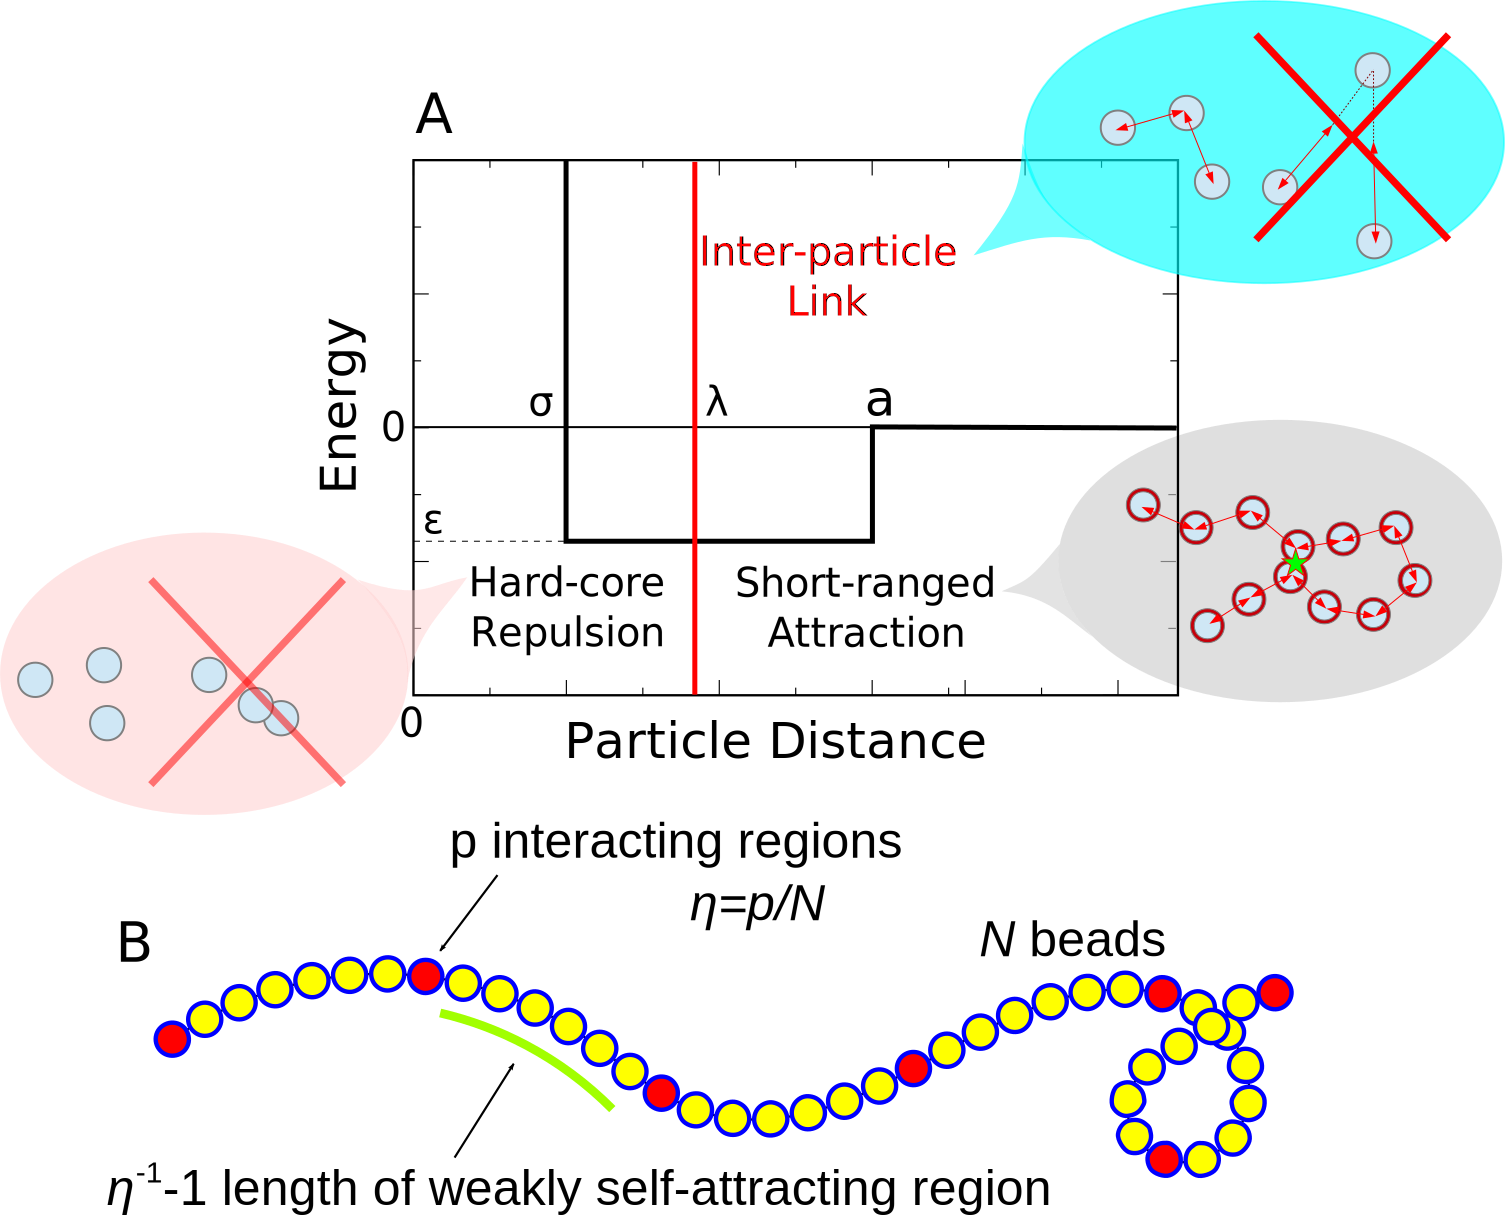
\includegraphics[width=0.49\textwidth]{fig1}
 \caption{Illustration of the model. A: The interparticle potential
   comprises a hard-core repulsion between all discretization
   ``beads'' of the polymer (whose range is set by the parameter
   $\sigma$), and a short-ranged attraction potential of range
   $a$ and depth $\epsilon_u$ for the homogeneous self-attraction
   (acting on all beads) and $\epsilon_l$ for the sparse bridging
   interactions. Additionally, consecutive beads are subject to a
   maximum separation hard constraint of length $\lambda$.
%%
   B: Parameterization of the position of bridging interactions. A
   total of $p$ bridging beads are placed across $p$ equally spaced
   regions of length $\simeq N /p$. The beads in the interspersing
   regions only feel the weaker self-attraction of energy
   $\epsilon_u$. }
  \label{fig:1}
\end{figure}


The basic ingredients of the model are illustrated in
Fig.~\ref{fig:1}. Our simulation uses a simple off-lattice Monte Carlo
algorithm with Metropolis rejection rule. The algorithm is a variant
of the ``bead-spring'' polymer model of ref.~\cite{Cacciuto2006}. The
polymer is represented as a linear string of $N$ spherical ``beads''
of diameter $\sigma$, connected by bonds of maximal extension $\lambda
= 2.36 \sigma$ \textbf{(??? cacciuto mette 1.9)}. We simulated
polymers composed of up to 320 \textbf{???} beads.  All monomers
interact via a hard-core repulsion potential
\begin{displaymath}
  U_r(r_{ij}) = \begin{cases} 
    0,  & \mbox{if }\ r_{ij} > \sigma \\ 
    \infty, & \mbox{if }\ r_{ij} \leq \sigma \ . 
  \end{cases} 
\end{displaymath}
Additionally, consecutive monomers feel the nearest-neighbor bonds as 
\begin{displaymath}
  U_b(r_{i,i+1}) = \begin{cases} 
    \infty,  & \mbox{if }\ r_{i,i+1} > \lambda \\ 
    0, & \mbox{if }\ r_{i,i+1} \leq \lambda \ . 
  \end{cases} 
\end{displaymath}
The short-ranged attraction, between all monomers, is modeled as a
negative square well between the two bounds imposed by the two above
potentials, and within a maximum range of $a = 0.61\sigma$
(Fig~\ref{fig:1}A). The depth of the attractive potential is
$\epsilon_u$ for all beads, modeling a generic short-ranged attraction
due to depletion effects / molecular crowding~\cite{Noro2000}.
Bridging interactions are represented by a square-well attractive
potential of the same range, but with interaction energy $\epsilon_l >
\epsilon_u$, for sparsely chosen beads.
%

%%%
%%%
Fig.~\ref{fig:1}B illustrates the criteria for placing the bridging
interactions and their parameterization. We considered a situation
where bridging regions are sparse and defined by the parameters $p$,
the number of bridging regions, and $\eta=p/N$ is the total fraction
of beads occupied by the bridging regions. We are interested in the
regime where $\eta$ is small. 
% This parameterization is invariant with respect to the number of
% statistical units $N$ representing the polymer.




\section{Results}

%%%% FIGURE

\subsection*{Collapse from homogeneous self-attraction. }

%%% and parameter  estimate.

\begin{figure}
  \centering
  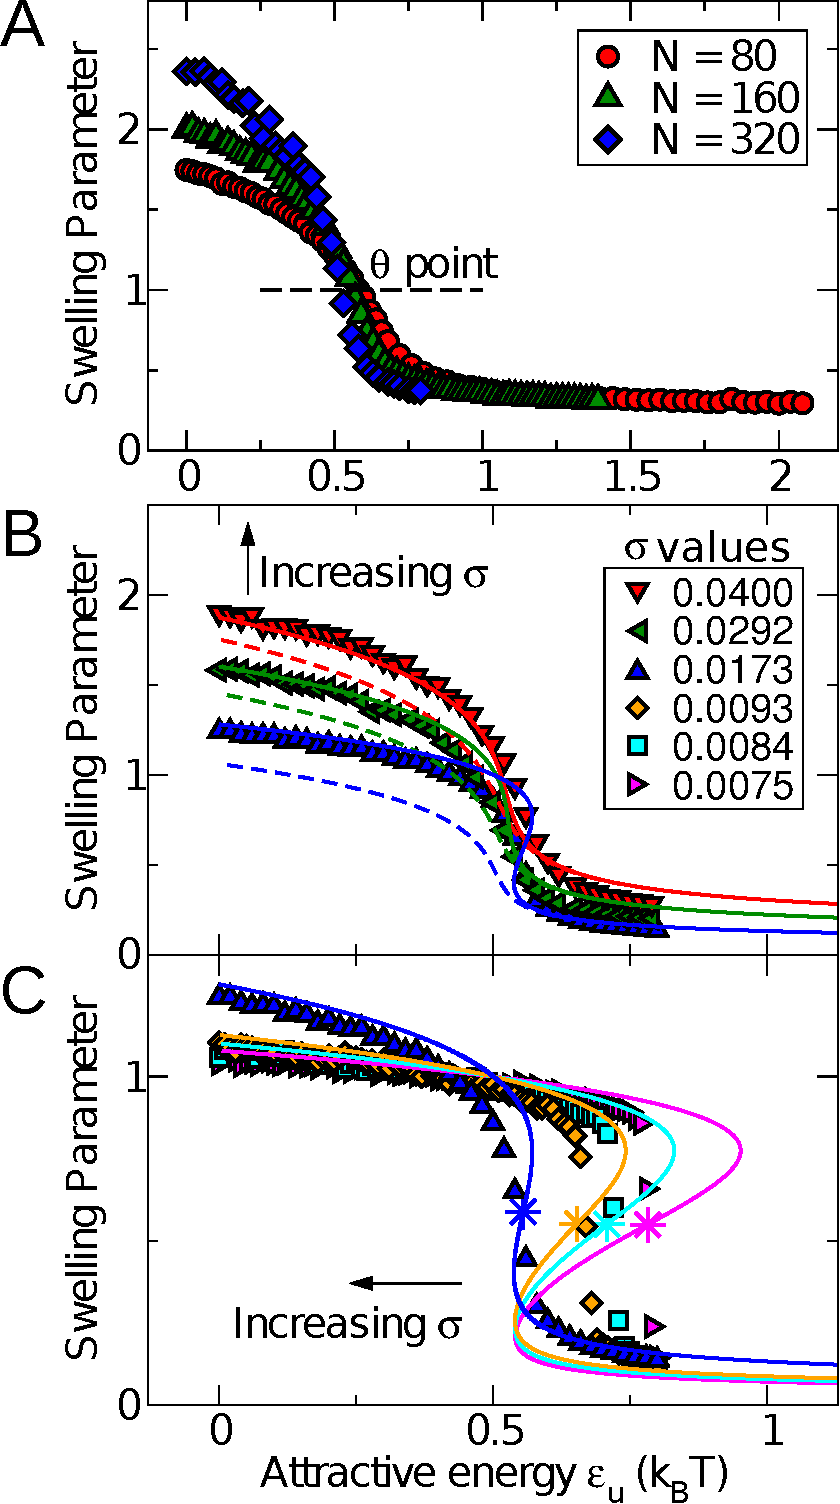
\includegraphics[width=0.4\textwidth]{fig_2}
  \caption{Collapse under homogeneous short-ranged attraction and
    mean-field theory. A: Collapse curve of the swelling parameter
    $\alpha$, plotted as a function of the attraction energy
    $\epsilon_u$, for different values of $N$. B and C: Comparison of
    collapse curves with mean-field theory for polymers with different
    excluded volume (varying $\sigma$) and $N=320$.  Solid lines are
    solutions of the modified mean-field theory,
    Eq.~(\ref{eq:deg_mfield}), while dashed lines are solutions of the
    standard mean-field theory. Panel C shows that for small values of
    $\sigma$ the inflexion point of the collapse curve becomes very
    steep, and moves towards larger values of $\epsilon_u$
    energy. This feature is qualitatively captured by the modified
    mean-field theory. We observed that the numerical collapse points
    match the reentrant inflexion points of the theoretical curves
    (indicated by stars on the solid lines in the plot.  }
  \label{fig:2}
\end{figure}


As a test scenario, we first considered the limit case of collapse of
a simple polymer with homogeneous self-attraction (a homopolymer). In
this case one expects to find the conventional theta transition, and it
is the case in our simulations. To show this, we considered the
swelling parameter $\alpha$, defined here as the ratio of the mean
end-to-end distance of the polymer $R_e=\langle |\mathbf{r}_N -
\mathbf{r}_1| \rangle$ in a given condition and its value $l_0=
lambda N^{1/2}$
%\textbf{perche' $3/5$? } 
% perche' \int_0^1 4 \pi r^4 dr / \int_0^1 4 \pi r^2 dr = 5/3
% comunque il concetto e` quello di far si` alfa al theta point sia
% uguale ad 1 e mi sembra gia` chiaro cosi`
at the theta point.  Fig.~\ref{fig:2}A shows a plot of this quantity
as a function of the homogeneous self-attraction energy per bead
$\epsilon_u$, for polymers with increasing $N$. The theta point is
located where the swelling parameter equals one.  We verified that its
position corresponds well to the prediction of the Flory mean-field
theory, which defines the theta point from the balancing, in the
second virial coefficient, of the excluded volume interaction term
with the attraction term. In our case both terms can be estimated from
the Mayer function, respectively as $v_1 = 4/3 \pi \sigma^3$
(repulsion) and $v_2= 4/3 \pi \beta \epsilon_u (a^3 - \sigma^3)$
(attraction), with $\beta=1/(k_B T) $.


The theta point is not the only relevant reference point for the
collapse. This is evident considering the collapse curves of the
swelling parameter for varying excluded volume (Fig.~\ref{fig:2}),
i.e. varying $\sigma$.  As $\sigma$ increases, the theta point
correctly shifts towards larger energy values (Fig.~\ref{fig:2}B).
%%
However, for increasingly ``thin'' polymers, while the theta point
still follows the predicted behavior, the inflexion point of the
swelling parameters vs $\epsilon_u$ curve becomes very steep, and
radically moves towards increasingly larger values of $\epsilon_u$
instead of smaller ones. These values, and not the theta point, are
where the ``collapse'', intended as a major jump in the swelling
parameters, effectively takes place.
%%
This phenomenology has been reported previously~\cite{DeGennes1975},
and may correspond to a first-order transition related to polymer
crystallization~\cite{Taylor2009}.


%%%% 
% Mean-field theory for collapse transition in absence of BPs 
%%
% 
The commonly used way to find the globule size and reproduce the
collapse curve by a Flory-like mean-field theory is to counterbalance
the two-body interaction term described above with a three-body
excluded volume term. We find improved agreement with the following
variant~\cite{DeGennes1975}
  \begin{equation}
    \beta F = 3 [\alpha^2/2 - log \alpha] + N/2 [B_1 \rho  + B_2 \rho^2 ] \ ,
    \label{eq:deg_mfield}
\end{equation}
where $\rho = N/R^3$ is the concentration, $B_1 = v_1 - v_2$ and $B_2
= (v_1)^2 / 6$. Note the logarithmic entropic term
coming from the prefactor of the radial distribution of a
freely-jointed chain.
%
% Or it comes from the enthropic cost of making a globule due
% to the contact probability?
%
This term becomes relevant for $\alpha < 1$ and its
addition is sufficient to capture the behavior described above.  For
extremely small excluded volumes, this mean-field theory also fails
quantitatively (Fig.~\ref{fig:2}C), but we noticed that (for
unexplained reasons) the reentrant inflexion points of the theoretical
collapse curve correspond remarkably well to the collapse points
observed in our simulations.



% IN APPENDIX ???? 
%
%%%% Matching of the parameters with collapse transition
%
%


\subsection*{Collapse in presence of bridging interactions}



\begin{figure}
  \centering
  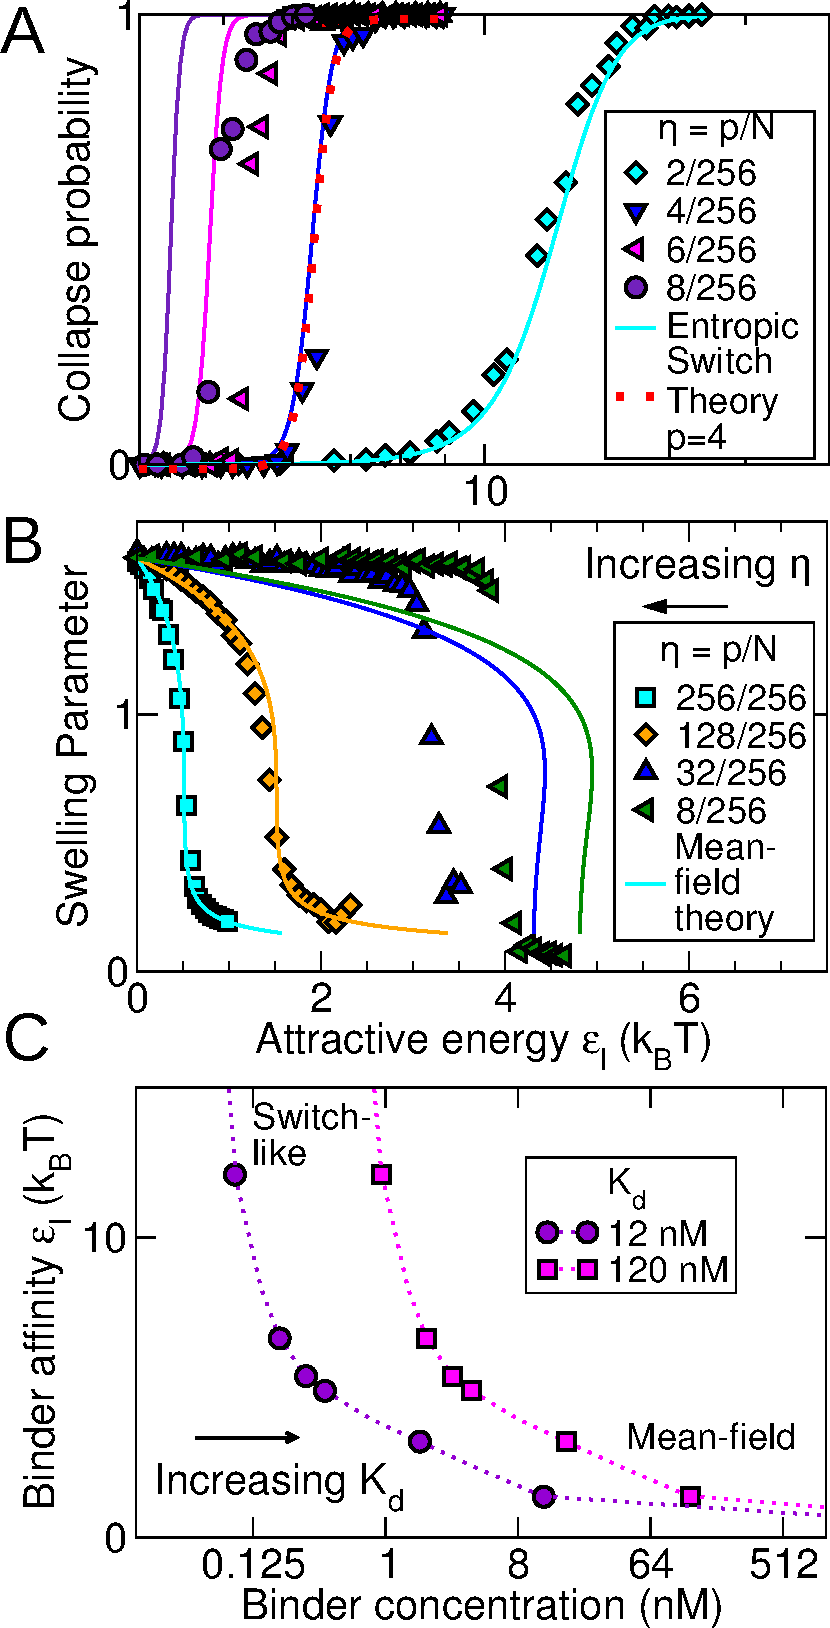
\includegraphics[width=0.4\textwidth]{fig3}
  \caption{Collapse due to bridging proteins.  A: Switch-like
    transition to a collapsed state for polymers with $p=4$ and $N=256$.
%
B: Collapse curves (swelling parameter vs
    $\epsilon_l$) drawn for different fractions of bridging
    interactions $\eta$; the transition energy moves to lower values
    for decreasing $\eta$ (coded by color and symbols, see legend),
    the case $\eta=1$ corresponds to the case of uniform collapse. The
    parameters have been chosen so that the phenomenology of
    Fig.~\ref{fig:2}C is not present. 
%%
C:  Transition energy plotted as a function of an effective
concentration  of bridging proteins, estimated  from $p,N$, by a
simple 
Langmuir model. We assumed a dissociation constant $K_d\simeq 0.5
\mu$M 
for the binders \textbf{check this use muM for the x axis}.      
%
% Simulations are  
% performed varying $\eta$ and $\epsilon_l$, with fixed $\epsilon_u = 0$
% and  \textbf{FIX HERE!}
% $N = 256$, $\sigma= $ $\lambda = 1/N^(1/2) l_0$.
% % eta/p=0.250/32   
% % p = 4,8,16,32,64 for panel C
% %
% \textbf{1 column - panel B becomes inset / show alpha shoulder /
% small % text/symbols and general visibility problems. H-NS $\to$
% Bridging % complexes $\Chi \to S_l$}
}
  \label{fig:3}
\end{figure}

%%% CITARE / VEDERE MARENDUZZO MICHELETTI 
%
% vedi entropy-driven genome org : c'e' argom.

We now discuss the case of collapse driven by sparse bridging
interactions only ($\epsilon_u = 0$). This case is sometimes presented
as analogous to the classical collapse transition of a
homopolymer~\cite{Barbieri2013a}. While we confirm this analogy, we
also find that there are important physical differences between the
two situations. The conventional theta point and collapse are
determined essentially by a balance between excluded volume and
attractive interaction. In presence of sparse bridging points, the
relevant contribution balanced by attractive energy is not monomer
excluded volume, but rather the entropy reduction for closing loops
between bridging points. In order to show this, we have considered
explicitly the following simplified partition
function~\cite{Marenduzzo2006c,Saiz2006a},
\begin{equation}
  \label{eq:Zloop}
  Z = \sum_{C} d_C e^{-\beta n_b^{(C)} \epsilon_l + \Delta S(C)} \ ,
\end{equation}
where $C$ runs over the possible bridging states, with degeneracy
$d_C$
%%% (see Appendix XXX)
%%% da decidere se fare un'appendix in cui spieghiamo un po' meglio
and $n_b$ is the number of bridging interactions, estimated as the
number of pairs of interacting bridging monomers in a given
configuration. For example, for $p=4$, $n_b^{\mathrm{(min)}}=0$,
$n_b^{\mathrm{(max)}}=6$. In general, if we would ignore the effect of
hard core repulsion and finite length attractive interactions we would
obtain $n_b^{\mathrm{(max)}}=p(p-1)/2$ while in presence of hard core
repulsion the term grow linearly with $p$.
%
There is only one ``fully collapsed'' state $C^*$ (we neglect in
this argument for simplicity surface effects in the core, see
below). The probability for such state is:
\begin{equation}
  \label{eq:prob_collapseZ}
  P(C^*) = Z^{-1}  e^{-\beta n_b^{\mathrm{(max)}} \epsilon_l + \Delta S(C^*)}
\end{equation}

To estimate the entropy loss contributions for each loop, one can
simply use the first return probability of a ghost chain (random walk)
of length $g\simeq N/p$. This is estimated, for large $g$, as
$P_\mathrm{(loop)}\simeq (2\pi g)^{-3/2}$. This term can also be
corrected for self-avoidance effects giving the mean-field estimate
$P_\mathrm{(loop)}\sim g^{-9/5}$. For both estimates, the entropy of a
single loop is $\Delta S_1(g) \sim \log g$. 
%
While the entropy of many configurations can be estimated as a
combination of loops of varying length, complex constrained
configurations can emerge that are not reducible to simple loops, but
the entropy loss terms can be computed case by case in a
straightforward way (for example for $p=4$ only one such configuration
emerges, connecting bridging points 1-3 and 2-4).  Fig.~\ref{fig:3}A
shows a comparison of the calculation carried out for $p=4$, and
direct simulation.  The agreement between the estimated and measured
$P(C^*)$ is very satisfactory, indicating that indeed a loop entropy
reduction switch is relevant as expected.
%
Additionally, we find that for $\eta=p/N$ sufficiently small, the
dominant contribution to the estimate is the collapsed one $C^*$, and
the transition can be captured by a simplified two-state partition
function keeping into account only the fully unfolded and the fully
bridged configurations (Fig.~\ref{fig:3}A),
\begin{equation}
  Z_R = 1 +  e^{-\beta n_b^{\mathrm{(max)}} \epsilon_l + (p-1) \Delta S_1(g)} \ .
  \label{eq:Zloop_red}
\end{equation}
This kind of switch-like looping transition has been studied in the
context of transcriptional regulation~\cite{Saiz2006a}.

%
Fig~\ref{fig:3}B shows the observed collapse curves for the swelling
ratio for different densities of bridging interactions $\eta$. There
is a crossover between the switch-like behavior just discussed and the
classical homopolymer collapse behavior (as shown in
Fig.~\ref{fig:2}), which naturally emerges when $\eta$ is sufficiently
large. This problem has been addressed classically: for example, a
transition from collapse to freezing has been found for $\eta \simeq
0.6$~\cite{Camacho1997}. However, we are not aware of existing studies
characterizing the crossover between a switch-like and mean-field-like
collapse. While we have not explored systematically this crossover, we
find that in our simulations polymers show mean-field collapse for
values of $\eta$ around ROUGH NUMBER \textbf{check this: per mettere questo
  numero controlla a occhio per che valori di eta la teoria mean field
  comincia a pigliarci decentemente...}.
%%


%%%%%%%%%%%%%%%%%%

Finally, Fig.~\ref{fig:3}C makes a parallel between the case of
sparse bridging interactions with no homogeneous self-attraction, and
the ``strings and binders switch'' (SBS) model used in the context of
eukaryotic chromatin~\cite{Barbieri2012,Barbieri2013b}.
%%%
The only difference between the two situations is that in the SBS
model a pre-defined set of sparse bridging interactions can be
occupied or not by a gas of bridging binders, while the set of
bridging locations is fixed in the model considered here. However, one
can map the two situations with a simple Langmuir process, assumed to
be in chemical equilibrium. We find that this operation leads to a
phase diagram that reproduces qualitatively the features of the SBS
model (Fig.~\ref{fig:3}C).



\paragraph*{Combination of sparse and homogeneous interactions} 


\textbf{DA FARE.} We now consider the case of collapse driven by both
sparse bridging interactions and homogenous self-attraction
($\epsilon_u > 0$).



\cite{Dasmahapatra2006}


\textbf{check this: servono  informazioni sulla mappa di contatto
  quando eps uniforme si avvicina alla transizione: vogliaos apere se
  un globulo collassato con energia di interaz discreta maggiore di
  uniforme e'  }



\begin{figure}
  \centering
  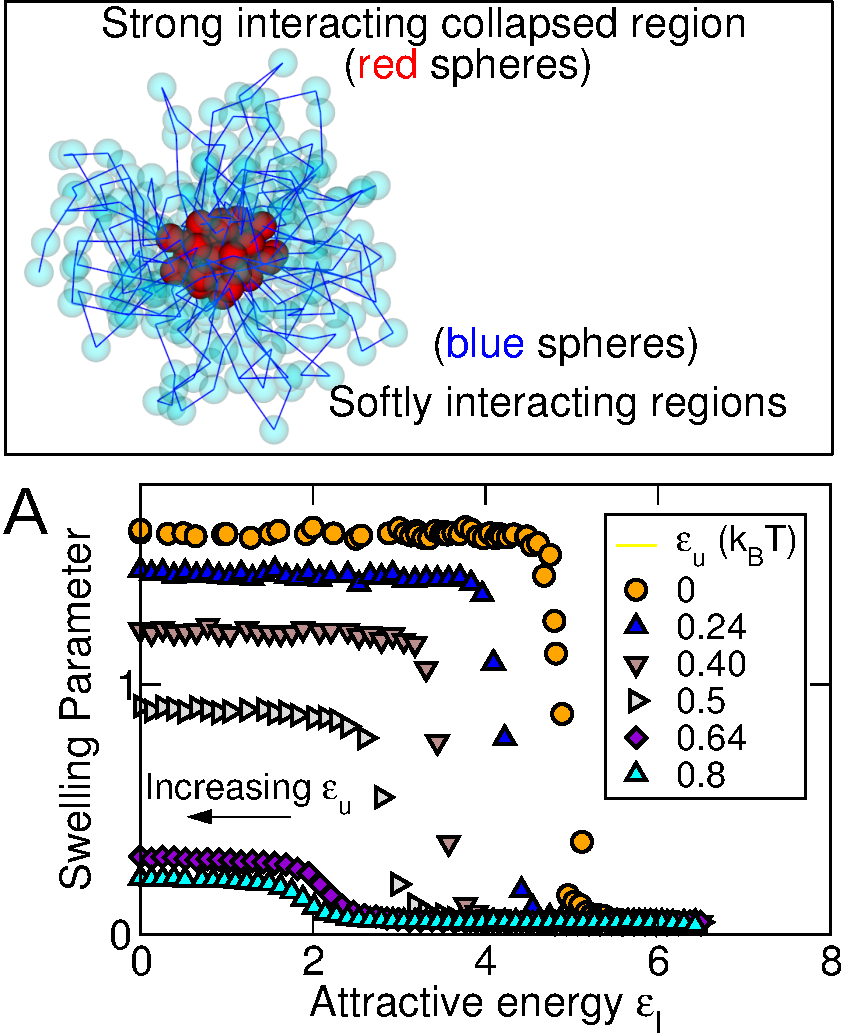
\includegraphics[width=0.4\textwidth]{fig4}
  \caption{\textbf{Da cambiare \\}Combined collapse from bridging
    interactions and uniform self-attraction.  A: Snapshot of a
    typical simulated collapsed configuration with bridging
    interaction stronger than uniform self-attraction. The collapse is
    driven by bridging, while the rest of the polymer forms closed
    (swollen or collapsed) loops \textbf{com'e' il caso in cui i loop
      uniformi non sono swollen ? lo puoi mostrare?}.
%%
    B: collapse curves ($\alpha$ vs $\epsilon_l$) shown for
    different values of $\epsilon_u$ (coded by color and symbols, see
    legend)
    % , the collapse occur at lower value of localized interaction
    % epsilon_l for higher epsilon_u,
    % simulations were performed with parameters (N = 256, Sigma =
    % (sigma^3*N) =
    % 0.0427611758752 l_0^3, Alpha = (alpha^3*N) = 3 Sigma, lambda =
    % 1/N^(1/2) l_0, p=32, eta=0.250 ).
%
    C: Adding uniform self-attraction (increasing $\epsilon_u$) shifts
    the transition point towards lower values of $\epsilon_l$ (see
    Fig.~\ref{fig:3}). }
%%%
% \textbf{Simulation parameters}
%     % Simulations are performed with parameters
%     % (N=256, Sigma = (sigma^3*N) = 0.0427611758752 l_0^3, Alpha =
%     % (alpha^3*N) = 3 Sigma, lambda = 1/N^(1/2) l_0, p=32)
% \textbf{Rename panels into A B C. small text/symbols and
% % general % visibility problems} }
  \label{fig:4}
\end{figure}


\subsection*{Compartmentalization}


Intriguingly, we find that the switch-like collapse, in the presence
of sparse interactions can lead to long-lived states where
\emph{multiple} collapsed domains exist. Fig.~\ref{fig:5}A shows a
snapshot of such a configuration. Multiple domains are visible from
interaction maps, i.e. tables where the indeces are the discrete
arclength coordinates of the polymer beads and the entries are
proportional to the probability of finding the two monomers within a
threshold distance \textbf{check this: le tue non sono queste - come
  hai definito le mappe??} (Fig.~\ref{fig:5}B). States with multiple
domains were stable in our simulations for as long as we could
measure. Additionally, states prepared with the initial conditions of
a single domain would switch to a two- or three-domain state, which
was then observed to be stable (Fig.~\ref{fig:5}B). This observation
leads us to believe that they might 
%
Additionally, the states can be observed also in presence of
homogeneous self-attraction, i.e. for $\epsilon_u>0$, and the
existence of such states affects the size and the shape anisotropy of
the collapsed globules, measured as the ratio between the first and
the third eigenvalue of the polymer's inertia matrix
(Fig.~\ref{fig:5}C). Evaluation of these quantities suggests that the
elongated configurations can be stable only if $\epsilon_u$ is such
that the polmer is above its theta point \textbf{check this manca
  valutazione diretta da mappa di contatto}.

In order to argue that multi-domain states could be stable, we rely on
the following scaling argument, related to the case of
polysoaps~\citep{Borisov1997,Borisov1996}. We consider a configuration
with $q$ domains, made of a ``core'' of $p/q$ bridging monomers and a
``corona'' of $p-1\simeq p/q$ loops.  Treating the loops of each
domain as a star polymer~\cite{Borisov1997} with $f=p/q$ ``arms'', and
knowing that the entropy of such an object scales as
$f^{3/2}$\cite{Daoud1982} leads to estimate the free energy change by
subdivision into $q$ domains as
\begin{equation}
  \Delta F_\mathrm{(corona)} \sim p^{3/2}q^{-1/2}
 \label{eq:poly1}
\end{equation}
The remaining relevant terms in the free energy are energetic, and
contain a core volume term (proportional to $\epsilon_l$) which is not
affected by the partitioning the polymer into domains, and the surface
tension term leading to the change
\begin{equation}
  \Delta F_\mathrm{(core)} \sim \epsilon_l (p)^{2/3}q^{-2/3} \ .
 \label{eq:poly2}
\end{equation}
Minimizing the two contributions with respect to $q$ (assumed
continuous) leads to the expected equilibrium number of domains 
\begin{equation}
  q_{\mathrm{eq}} \sim p  \epsilon_l^{-6/5} \ ,
\end{equation}
indicating that the number of stable domains should increase for
larger $p$ and decrease if $\epsilon_l$ is too large. 


This  behavior is observed in our simulations.  However, this
argument can be regarded as only qualitative. For example, a slightly
more precise evaluation of the entropy of a star polymer leads to $
\Delta F_\mathrm{(corona)} \sim f^{3/2} \log\left(Nf^{1/3}/(b
  V_\mathrm{core}^{5/3}) \right)$, where $V_\mathrm{core}\sim q^{1/3}$
is the core volume. Equivalently, $ \Delta F_\mathrm{(corona)} \sim
p^{3/2}q^{-1/2} \log\left( p^{5/3}q^{-2/3} \right)$, which (even
neglecting prefactors) affects the predicted scaling. Additionally,
the argument for the entropy is consistent only when the arms are
above the theta point.
%%%
Note that, differently from the case of polysoaps, the multi-domain
states in this picture are due to the trade-off between the energetic
cost of the core surface when making multiple domains and the entropy
increase due to making star-like configurations with an increasing
number of arms.  Hence, according to the argument, a multi-domain
state is stable because partitioning $(p-1)$ arms into more than one
domain is less costly compared to the energy cost of partitioning the
bridging proteins in multiple domains.
  


\begin{figure}
  \centering
  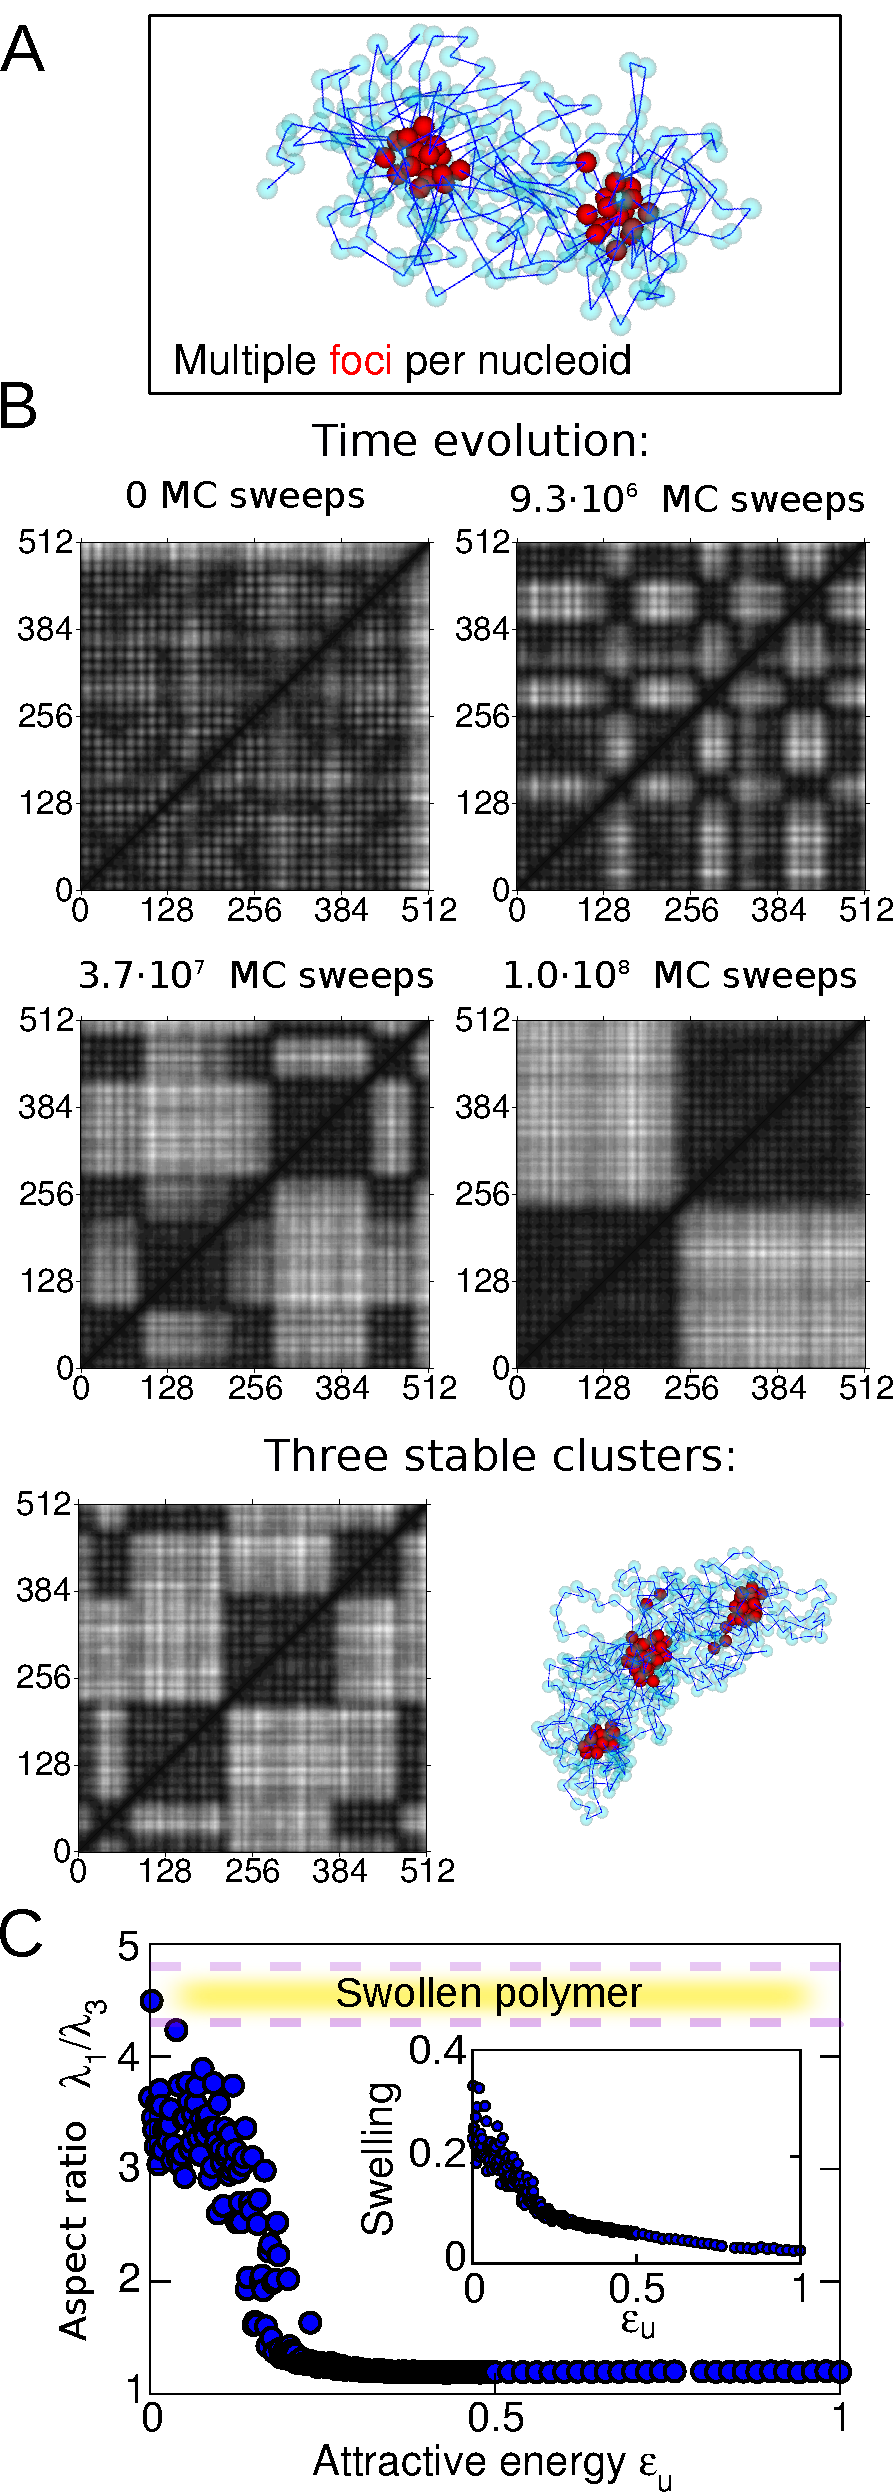
\includegraphics[width=0.4\textwidth]{fig5}
  \caption{Self-assembled micro-segregation into domains and shape
    anisotropy.  A: Snapshot of a typical two-domain configuration;
    the two domains are stable due the entropic repulsion of the
    loops arranged in a star-like configuration.   
%
B: Stability of multi-domain configurations over single-domain
collapsed 
state. Colormaps of mean distance between polymer segments shown for
increasing Monte Carlo times.  
%
In lexicographic order:  (i)  initial configuration of the simulation 
prepared as a single domain (as in Fig.~\ref{fig:4}A), (ii) after
$2\cdot10^6$ 
Monte Carlo sweeps the system (simulated for
$\epsilon_l+\epsilon_u=2.4$, 
$\epsilon_u=0.15$)  shows a disintegration of the single-domain
configuration,  (iii) 
  at $10^7$  sweeps a two-domain configuration is stable;
  (iv)  different parameters    
($epsilon_l+epsilon_u=2.4$, $epsilon_u=0.005$) lead to a stable
three-domain 
configuration after $10^7$ sweeps.
%  
    C: The shape anisotropy of the collapsed globules (measured as the
    ratio between the first and the third eigenvalue of the inertia
    matrix)  shows a transition when the difference between the
    uniform  
    interaction  lower to a negative threshold. The
    transition is due to 
    the increasing repulsive interaction within the loops. The inset
    show that with  the same transition is visible  the volume-energy
    law.  \textbf{check this:  va 
      confrontata con l'anisotropia standard del swollen polymer,
      e bisogna segnare nel plot quando ci sono due domini e quando si
    passa a uno}. In these plots, 
    $\epsilon_l+\epsilon_u=3.4 K_b T$ \textbf{perche' scelgi di
      conservare la somma?}.  
%
\textbf{Simulation parameters. }
Simulations are performed with $N = 512$, $sigma =$ 
 $lambda =$   $p=32$, $eta=0.125$, $l_0= $.  
%
\textbf{Change colorscale of interaction map. Rename panels into A B
  C, invert panels C ad B. small text/symbols and general visibility problems} }
  \label{fig:5}
\end{figure}





% \subsection*{Phase diagram}


% \begin{figure}
%   \centering
% %  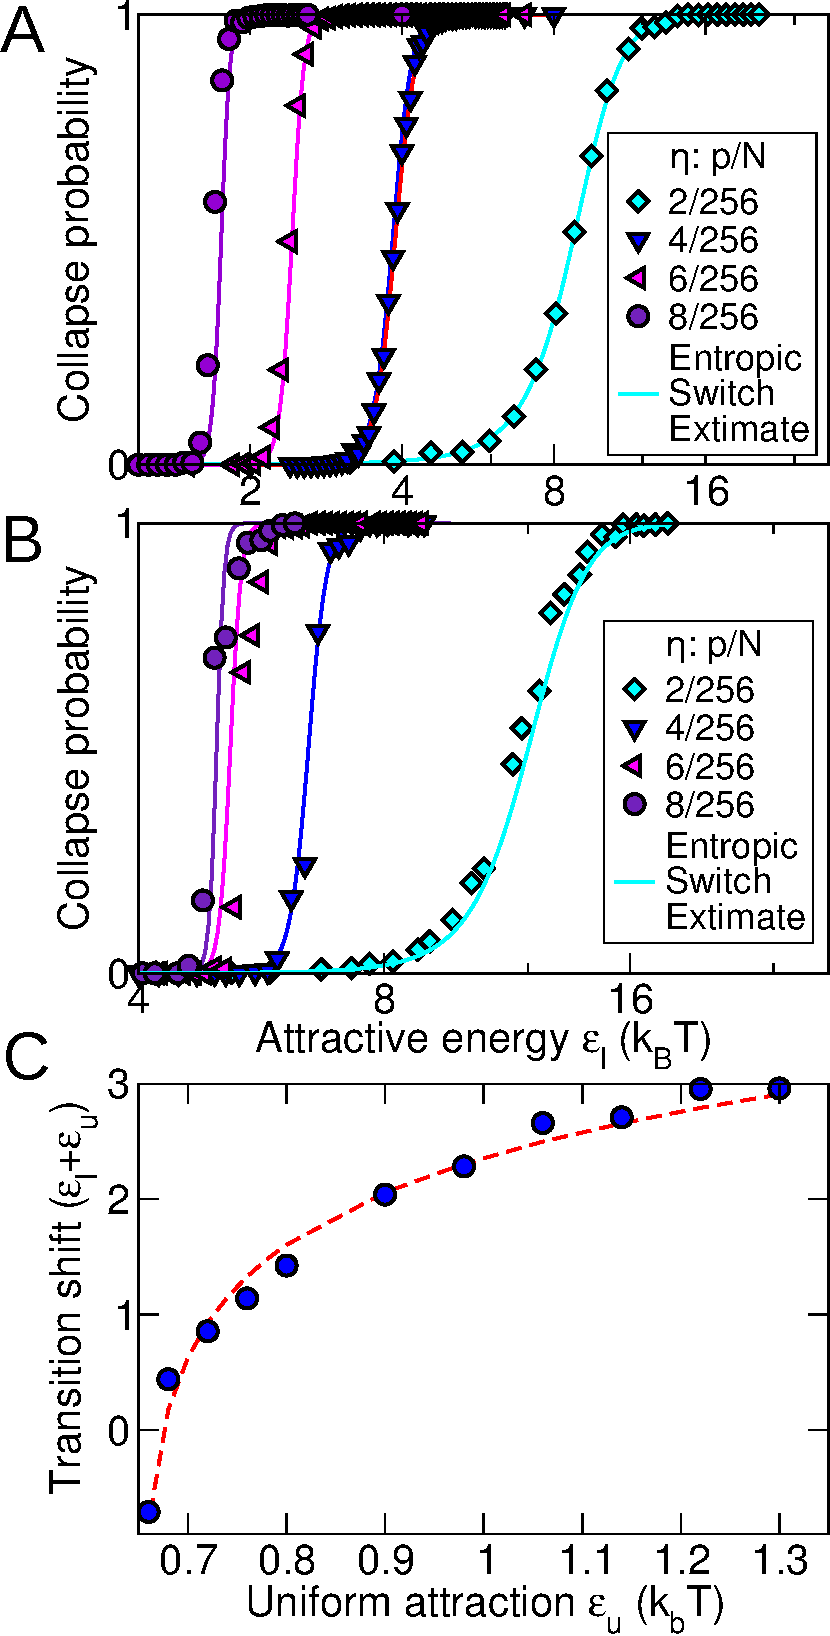
\includegraphics[width=\0.9columnwidth]{fig6}
%   \caption{Qualitative phase diagram of the model. }
%   \label{fig:6}
% \end{figure}


\section{Discussion. }
\label{sec:Disc}


While computational models that describe well several aspects of
bacterial and eukaryotic chromosome organization are abundant,
theoretical arguments helping understand the behavior and place it in
the framework of known polymer physics.  
%%
In this study, we considered the case of polymer collapse driven by a
combination of homogeneous and sparse attractive interactions, and
made an effort to capture the observed phenomenology by developing
quantitative scaling arguments and simulation in parallel. 
%%
Additionally, we connected the main results found here with related
findings in different sectors of the polymer physics literature. 

The simple model of compaction

% OTHER INGREDIENTS


%%% LINEAR ORDERING
% For cells that are not replicating the genome, the position of
% genetic loci along the chromosome is linearly correlated with their
% position in the
% cell~\cite{Viollier2004a,Breier2004,Wiggins2010}. The exact
% subcellular positioning of different loci varies in different
% bacteria~\cite{Toro2010}.
%
% usa hp polysoap


%%% SUPERCOILING
There is another possibly important ingredient,
supercoiling/branching, which we disregard for simplicity. Reasons why
we can disregard it?

What could it do? Modulates the loop entropy and the loop
probability. Changes the contact map. Affects the radius of gyration
at fixed conditions.

%%% ENTANGLEMENT
%% Beyond the reach of the simulation method.
%%
% 
%
%




%%% SEGREGATION & NONEQ ASPECTS 
Finally, we have assumed that an equilibrium model can give some
insight into the process of bacterial chromosome organization. While
this might be true at certain time- and lenght-scales, we note that
non-equilibrium aspects are emerging as an important feature of
nucleoid organization.  Firstly, on the time scale of cell division
the chromosomes segregate following a well-defined
``choreography,''~\cite{Youngren2014,Fisher2013,Kuwada2013,Toro2010}.
%
% During replication, daughter chromosomes demix and segregate before
% cell division. In \emph{ E.~coli}, the two arms of the chromosome
% are segregated in an organized $<$left-right-left-right$>$
% asymmetric fashion from the center of the
% cell~\cite{WLP+06,NYH+07,Toro2010}. Replicated chromosomal loci are
% thought to be immediately recondensed, as they appear to preserve
% the linear arrangement while they are moved in opposite directions
% to assume their final position in the incipient daughter
% cell~\cite{Thanbichler2005,Thanbichler2006}.
Secondly even on very short time scales, different non-equilibrium
active phenomena are reported, including non-thermal loci
motion~\cite{Weber2012a}, longitudinal compression
waves~\cite{Fisher2013} and very rapid transitions driving segregation
itself ``snaps''~\cite{Fisher2013,Joshi2011,EMB08}.  Such processes
are they are beyond the reach most available polymer-physics modeling
approaches used to investigate the nucleoid.



%%\section{Conclusions. }


%%%%%%%%%%%%%%%%%%%%%%%%%
\begin{acknowledgments}
  We are very grateful to Peter Olmsted, Mario Nicodemi, Emanuela del
  Gado, Bianca Sclavi
%%% ALTRI (?) 
  for discussions, useful feedback, and to
%%%%
  comments on this manuscript.  This work was supported by the
  International Human Frontier Science Program Organization, grant
  RGY0069/2009-C.
\end{acknowledgments}



\bibliography{bibs_bridge}    


\appendix

\section{Scaling procedure for matching the parameters with
  experimental data}


%%%% qui teoria riscalata e stima parametri


% By choice, the description is invariant by rescaling, and different
% numbers of beads are just different discretizations of the same
% reference (finite) object

% NB: edwards model does not admit well-defined continuum limit and
% likely this holds for this model too.

% Different from standard choice in polymer physics, but useful in
% modeling context, as we can think of different discretizations as
% increasingly finer descriptions of the same object.
  

% %
% Matching of the parameters with the bacterial nucleoid [this could
% be here, or, if we expand it, at the end, in the results]

% \section{}
% more details on switch argument?
%

\section{Scaling argument for the entropy of a star polymer.}

These notes describe the calculation of the number of blobs of a star
polymer with $f$ arms, each of length $N$, bridging some implicit
parts of the calculation carried out by Daoud and Cotton (1982). The
number of blobs can then be used as a proxy for the entropy (blob
ansatz).

The polymer is described as a series of concentric shells, each of
which by definition has to contain $f$ blobs (one for each
arm). However, the size of the blobs $\xi$ will depend on the radial
coordinate of the shell (called $r$). Since the shell at $r$ has
surface $\sim r^2$, the size of each blob is $\xi^2 = r^2/f$, which
means that $\xi \sim r / f^{1/2}$, i.e. $\xi = a r$, with $a = C
f^{-1/2} $.  $\xi$ is also the thickness of the shell at coordinate
$r$.


Starting form a core of size $r_0$ we now imagine to stack
(iteratively) discrete blobs of the proper size on each shell. Each
stacked shell will determine the coordinate of the following one, and
hence its blob size. We thus write
\begin{displaymath}
  r_i = a \sum_{k=1}^{i-1} r_k + a \frac{r_i}{2} + a r_0 \ ,  
\end{displaymath}
with
\begin{displaymath}
  \xi_i = \xi(r_i) = a r_i \ .
\end{displaymath}

Immediately one has 
\begin{displaymath}
  r_i \left(1 -\frac{a}{2} \right) = a \sum_{k=0}^{i-1} r_k
\end{displaymath}
i.e. 
\begin{displaymath}
  r_1 \left(1 -\frac{a}{2} \right) = a r_0
\end{displaymath}
\begin{displaymath}
  r_2 \left(1 -\frac{a}{2} \right) = r_0 a(1+a)
\end{displaymath}
\begin{displaymath}
  r_n \left(1 -\frac{a}{2} \right) = r_0 a (1+a)^{n-1} \ .
\end{displaymath}

and
\begin{displaymath}
  \xi_n = r_0 a^2 (1+a)^{n-1} \ .
\end{displaymath}

We note now that the relationship $\xi_n \sim g_n^{3/5} v^{1/5} b$,
also has to hold (each blob is a swollen polymer of bond length $b$),
where $v=1/2 - \chi$, and $g$ is the number of monomers in a
blob. Hence,
\begin{displaymath}
  g_n = A e^{\frac{5}{3}\left(n-\frac{1}{2}\right)a} \ ,  
\end{displaymath}
where
\begin{displaymath}
 A= \frac{(a^2 r_0)^{5/3}}{v^{1/3} b^{5/3}} . 
\end{displaymath}

The important part is that  
\begin{displaymath}
  g_n \simeq A e^{\frac{5}{3}n a} \ ,  
\end{displaymath}
for $n$ sufficiently large.

We now follow (on one branch of the star) all the monomers in all the
blobs, and impose that their total has to be $N$. Inverting this
relationship will give an estimate for $N_{\mathbf{blob}}$. This can
be used to estimate $\beta F \simeq f N_{\mathbf{blob}}$ (since the
argument only involves the blobls of one arm).

One has
\begin{displaymath}
  \sum_{n=1}^{N_{\mathbf{blob}}} g_n = N \ ,
\end{displaymath}
hence
\begin{displaymath}
  N \simeq \int_{1}^{N_{\mathbf{blob}}} \mathrm{d}n  A e^{\frac{5}{3}n
    a} \ , 
\end{displaymath}
from which
\begin{displaymath}
  N_{\mathbf{blob}} \sim \frac{1}{a} \log N a / A
\end{displaymath}
where we neglected additive and multiplicative numerical constants

This leads to the final expression
\begin{displaymath}
  \beta F \sim f^{3/2} \log 
  \left(  N f^{7/6} v^{1/3}  \left(\frac{b}{r_0} \right)^{5/3} \right)
\end{displaymath}

Notes:

(i) The prefactor of $f^{3/2}$ is numerical and cannot contain $v$,
since it comes from the dimensionless expononent of $g_n$, which is
proportional to $n a$, and ultimately from the purely geometric
relationship $\xi^2 = r^2/f$.

(ii) Not sure about the exponent of $f$ in the log (last time I did it
I had one power less of a, giving exponent 1/3, but now it seems OK
this way...).

% \section{}
% more details on polysoap argument?



\end{document}

